\documentclass[11pt, a4paper]{article}

\usepackage[a4paper, margin=2.5cm]{geometry}
\usepackage[utf8]{inputenc}
\usepackage[T1]{fontenc}
\usepackage{float}
\usepackage{booktabs}
\usepackage{tabularx}
\usepackage{graphicx}
\usepackage{caption}    
\usepackage{pdflscape}   
\usepackage{hyperref}

\begin{document}
	
\begin{center}
	\vspace*{-1.5cm}
	{\LARGE\bfseries Trusting the Signal:}\\[4pt]
	{\Large\bfseries Explanation and Confidence in AI Investment Advice}\\[8pt]
	{\large\itshape Designing a buy/hold/sell assistant for appropriate reliance}\\[10pt]
	Ximin Chen \quad·\quad Student ID: 3085693 \quad·\quad University of Birmingham
\end{center}

\vspace{2pt}
\noindent\rule{\textwidth}{0.4pt}

\noindent\textbf{Word count:} ... words (abstract ...; main report ..., including the rationale table)\\
\textbf{Repository:} \url{https://github.com/CBsbisim/signal-assistant} (release \texttt{v1.0-a2})

\begin{abstract}
% Enter abstract text here.
\end{abstract}

\section{Problem and scope}

\section{Design Rationale Table}
\begin{table}[H]
\vspace{-1.5em}
\caption{Design Rationale Summary}
\centering
\begin{tabularx}{\textwidth}{l X X}
\toprule
\textbf{Design Aspect} & \textbf{Rationale} & \textbf{Status / Trade-off} \\
\midrule
% Add rows here, e.g.:
% Aspect 1 & Rationale description & Implemented \\
\bottomrule
\end{tabularx}
\end{table}
\section{Compromises}
\section{How it works}
\begin{figure}[H]
	\centering
	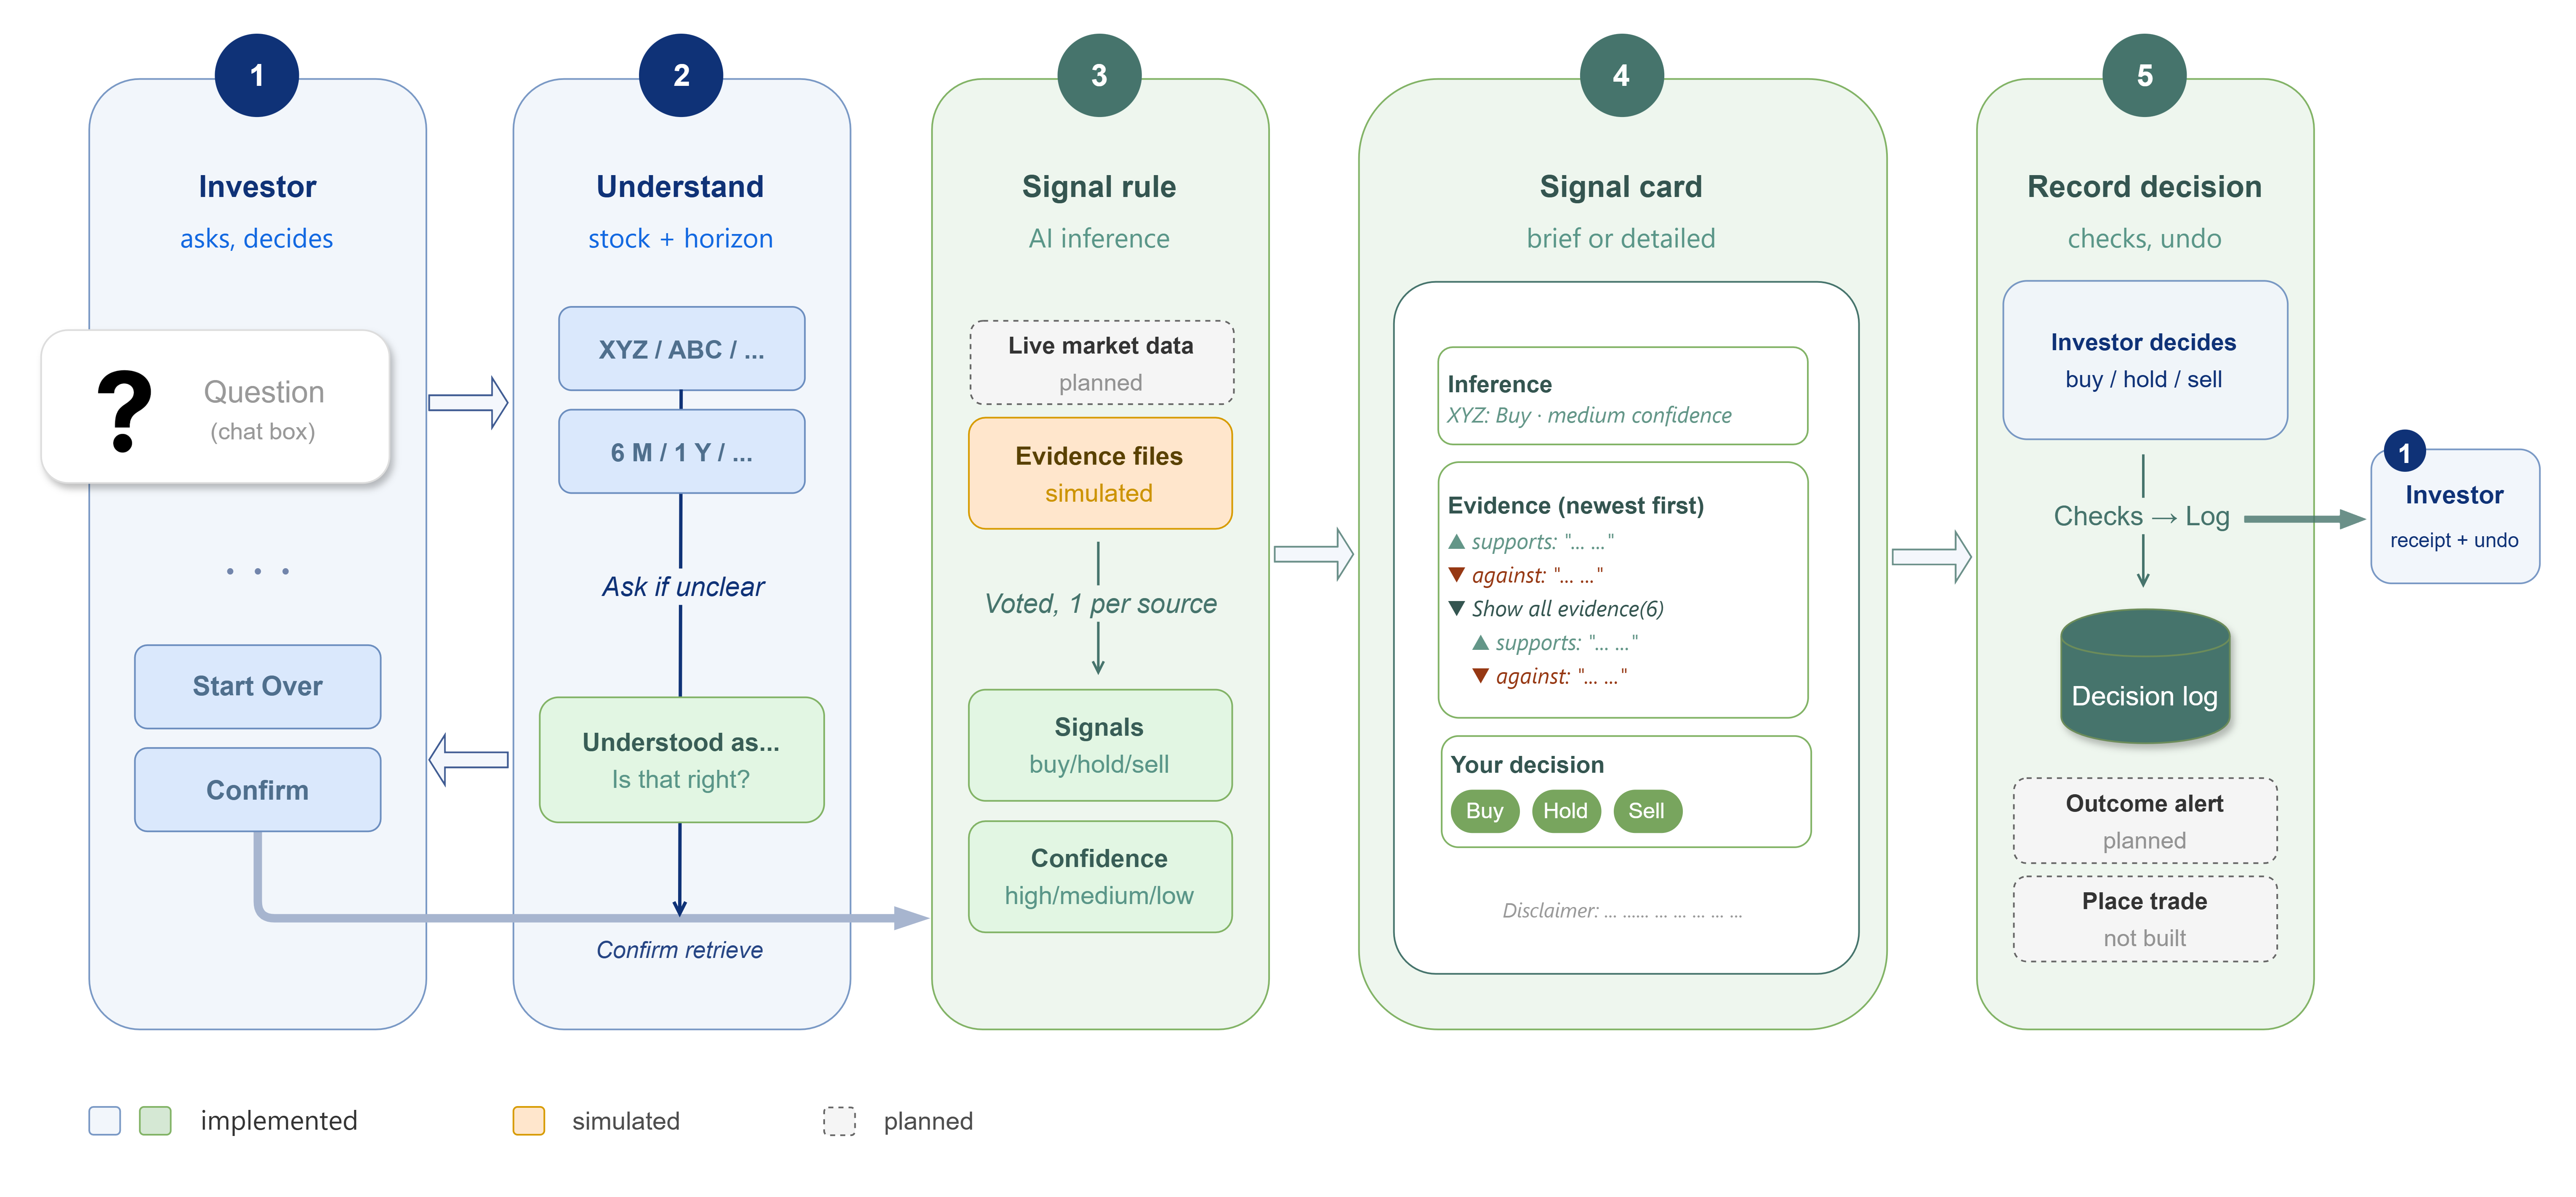
\includegraphics[width=1\textwidth]{images/system_diagram.png}
	\caption{System Architecture and Control / Data Flows}
	\label{fig:diagram}
\end{figure}
\section{Interaction examples}

\begin{landscape}
	\centering
	\includegraphics[width=\linewidth]{images/storyboard_1.png}
	\captionof{figure}{Storyboard 1: normal use. The person checks the evidence and decides against the signal.}
	\label{fig:sb1}
    \vspace{1em}
	\includegraphics[width=\linewidth]{images/storyboard_2.png}
	\captionof{figure}{Storyboard 2: recovery. The system asks instead of guessing.}
	\label{fig:sb2}
\end{landscape}

\begin{figure}[H]
	\centering
	\includegraphics[width=\textwidth]{images/storyboard_3.png}
	\caption{Storyboard 3: with one source, confidence stays low; the detailed view shows a single row.}
	\label{fig:sb3}
\end{figure}

\section{Development and testing}

\section{Repository and Development Evidence}

\subsection{Repository}
\url{https://github.com/CBsbisim/signal-assistant.git}

\subsection{Commit / Development History}
\url{https://github.com/CBsbisim/signal-assistant/commits/v1.0-a2}

\subsection{AI Assistance \& Authorship Accountability}
% Enter content for AI Assistance & Authorship Accountability.

\begin{thebibliography}{9}
% Add references here, e.g.:
% \bibitem{ref1} Author, \textit{Title}, Year.
\end{thebibliography}

\end{document}